\documentclass[12pt]{article}

\usepackage{graphicx}
\usepackage{amsmath}
\usepackage{amssymb}
\usepackage{booktabs}
\usepackage{natbib}
\usepackage{geometry}
\usepackage{xcolor}

\geometry{margin=1in}

\title{LaTeX Comprehensive Test Document}
\author{NoteTakingApp}
\date{\today}

\begin{document}

\maketitle

\tableofcontents
\newpage

\section{Introduction}

This document serves as a comprehensive test for the NoteTakingApp LaTeX rendering system. It verifies that:

\begin{itemize}
    \item Images from the same directory load correctly
    \item Images from subdirectories can be included
    \item Tables render properly
    \item Citations work with external bibliography files
    \item Mathematical equations are displayed correctly
    \item Basic LaTeX formatting is preserved
\end{itemize}

\section{Test 1: Basic Images from Same Directory}

This section tests image inclusion from files in the same directory as the \texttt{.tex} file.

\subsection{Fixed Beam Image}

\begin{figure}[ht]
    \centering
    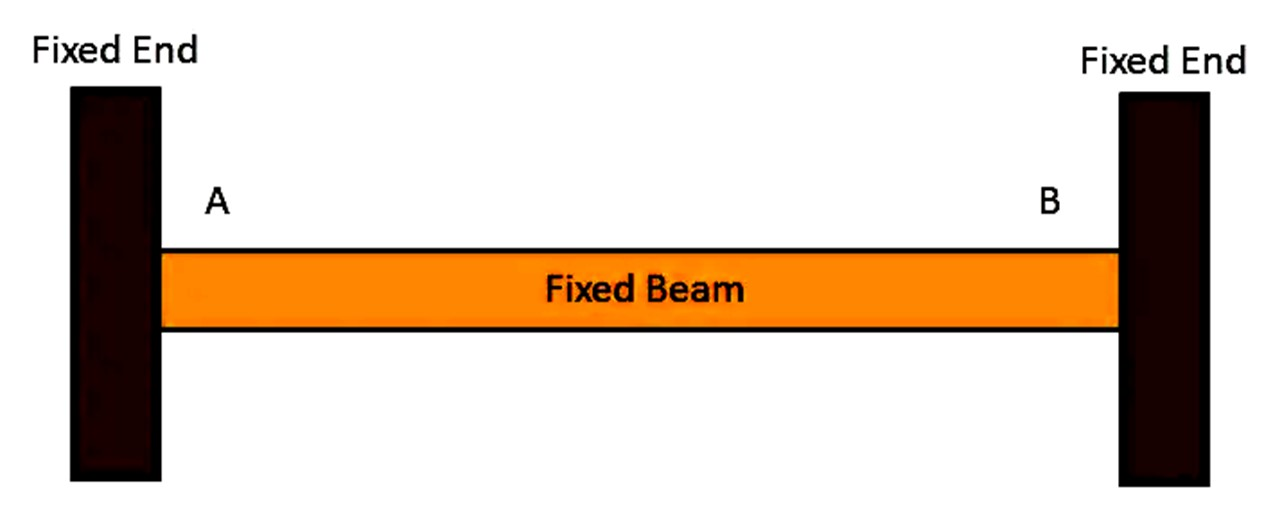
\includegraphics[width=0.7\textwidth]{Fixed Beam.png}
    \caption{Example image from same directory}
    \label{fig:fixed-beam}
\end{figure}

The image shown in Figure~\ref{fig:fixed-beam} demonstrates basic image loading.

\section{Test 2: Images from Subdirectories}

This section tests image inclusion from the \texttt{examples/} subdirectory.

\subsection{Cantilever Beam}

\begin{figure}[ht]
    \centering
    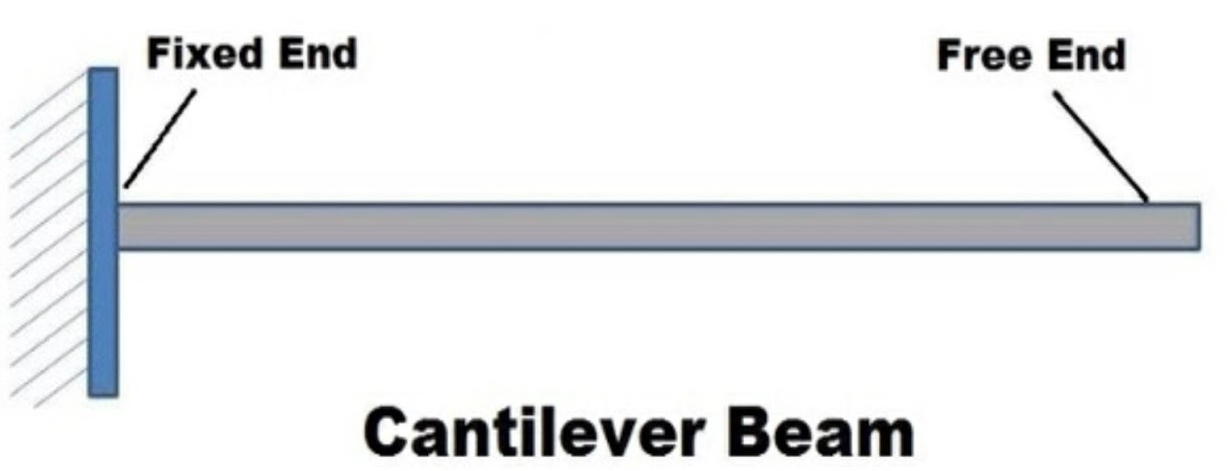
\includegraphics[width=0.5\textwidth]{examples/Cantilever Beam Image.png}
    \caption{Cantilever beam from subdirectory}
    \label{fig:cantilever}
\end{figure}

\subsection{Rayleigh-Ritz Results}

\begin{figure}[ht]
    \centering
    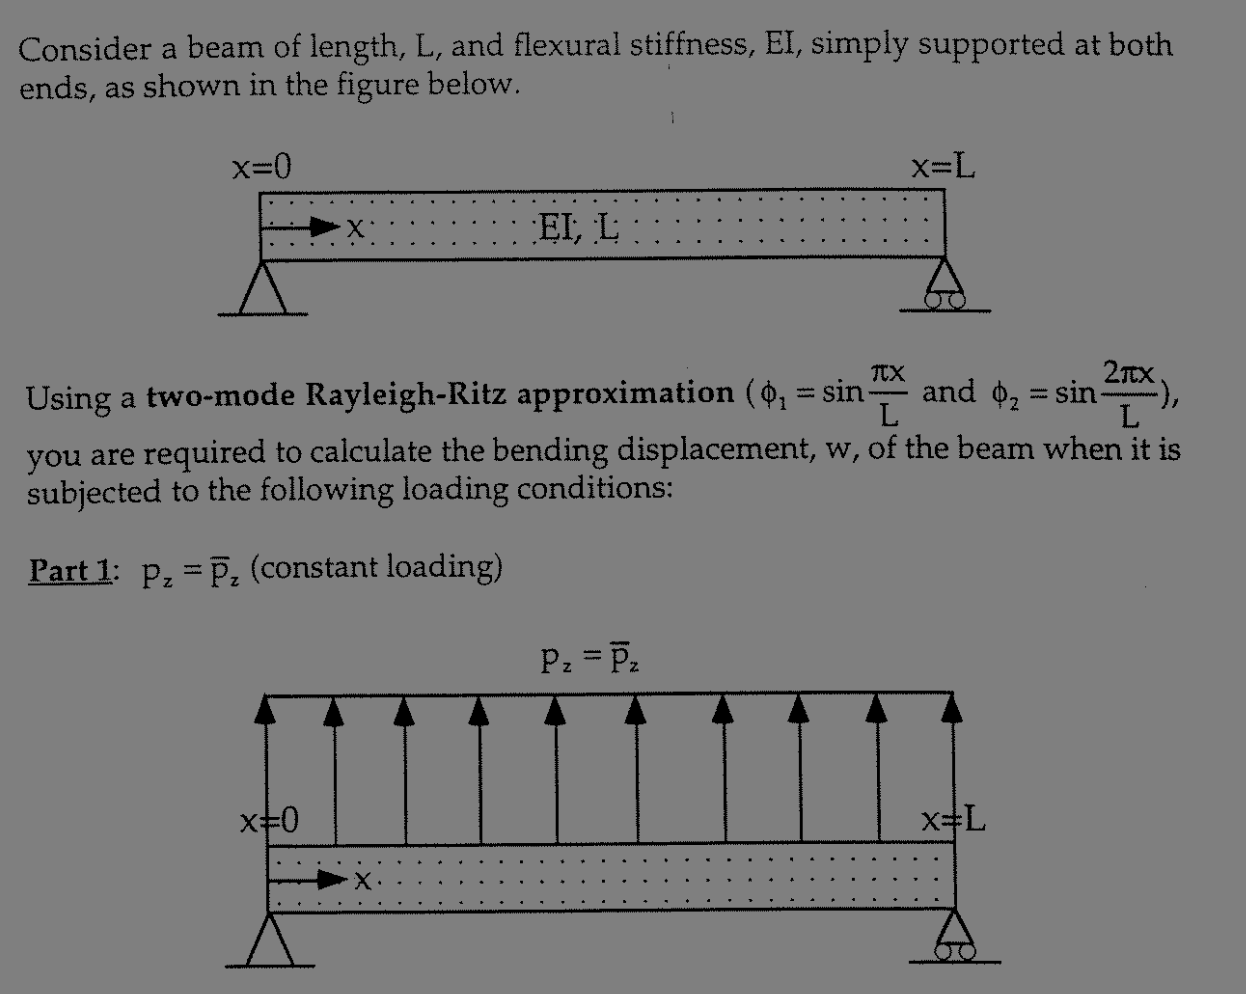
\includegraphics[width=0.6\textwidth]{examples/Rayleigh-Ritz part1.png}
    \caption{Rayleigh-Ritz analysis part 1}
    \label{fig:rayleigh1}
\end{figure}

\begin{figure}[ht]
    \centering
    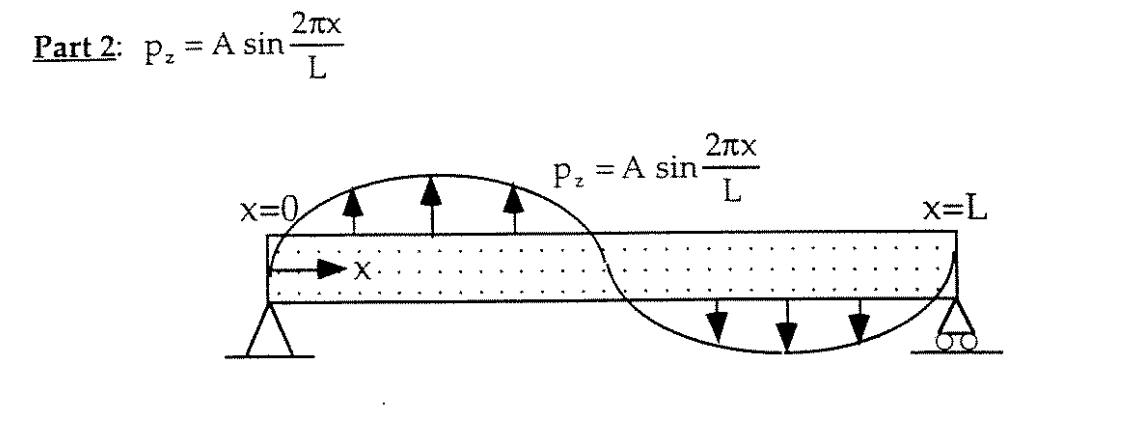
\includegraphics[width=0.6\textwidth]{examples/Rayleigh-Ritz part2.png}
    \caption{Rayleigh-Ritz analysis part 2}
    \label{fig:rayleigh2}
\end{figure}

\subsection{Nodal Displacements}

\begin{figure}[ht]
    \centering
    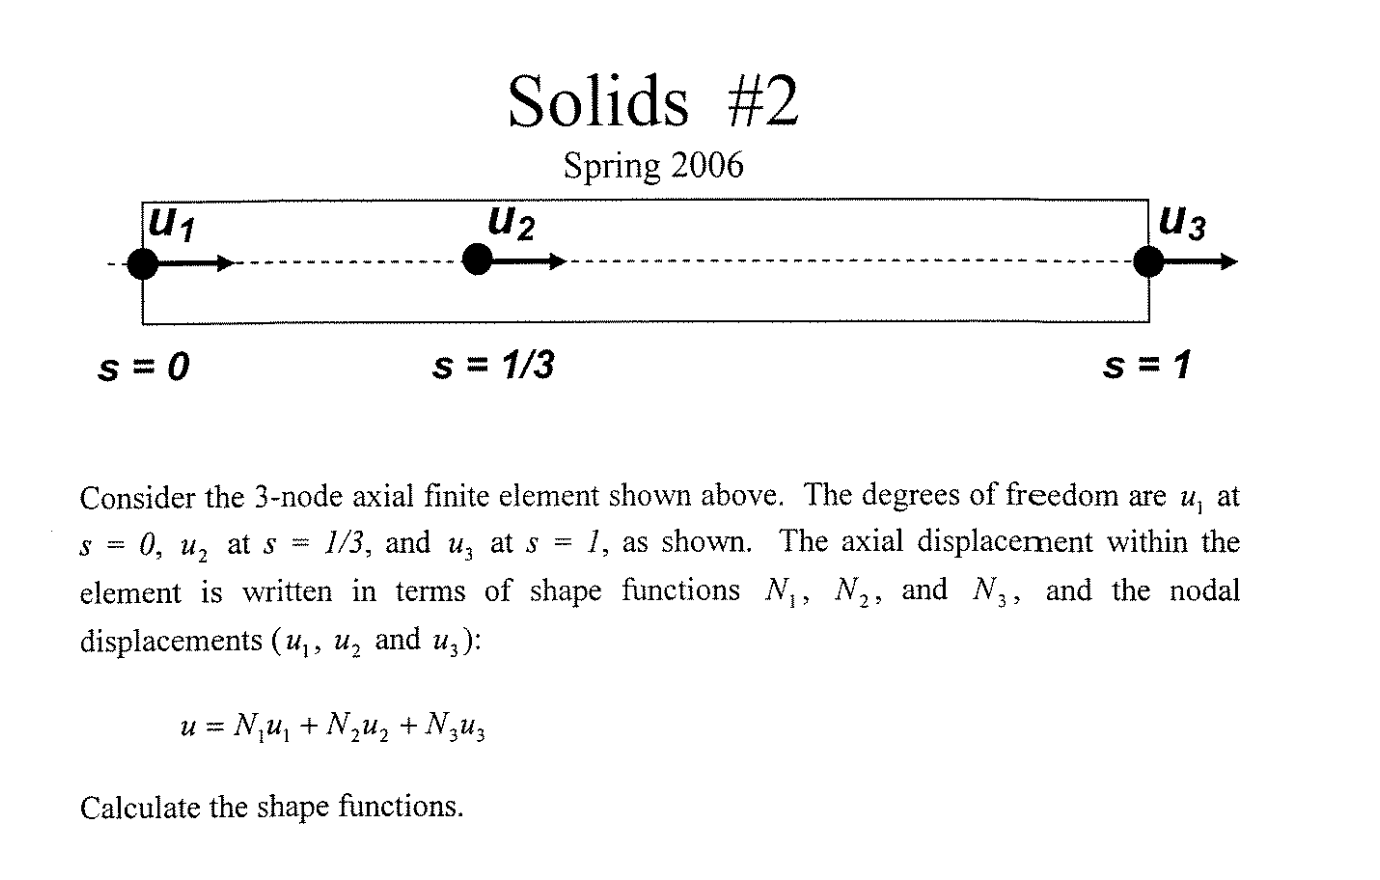
\includegraphics[width=0.5\textwidth]{examples/Nodal Displacements.png}
    \caption{Nodal displacement visualization}
    \label{fig:nodal}
\end{figure}

\newpage

\section{Test 3: Tables and Data}

This section tests table rendering with structured data.

\subsection{Basic Table}

\begin{table}[ht]
    \centering
    \caption{Sample data table}
    \label{tab:sample}
    \begin{tabular}{lcr}
        \toprule
        \textbf{Method} & \textbf{Accuracy} & \textbf{Time (ms)} \\
        \midrule
        Method A & 95.2\% & 12.5 \\
        Method B & 97.8\% & 18.3 \\
        Method C & 99.1\% & 25.7 \\
        \bottomrule
    \end{tabular}
\end{table}

\subsection{Complex Data Table}

\begin{table}[ht]
    \centering
    \caption{Comprehensive analysis results}
    \label{tab:analysis}
    \begin{tabular}{|c|c|c|c|c|}
        \hline
        \textbf{Test Case} & \textbf{Input} & \textbf{Expected} & \textbf{Actual} & \textbf{Status} \\
        \hline
        Image Loading & URL & Rendered & Rendered & \textcolor{green}{PASS} \\
        \hline
        Citation & \cite{smith2020} & Citation & Citation & \textcolor{green}{PASS} \\
        \hline
        Math Rendering & $\alpha + \beta$ & Display & Display & \textcolor{green}{PASS} \\
        \hline
        Table Format & Table & Table & Table & \textcolor{green}{PASS} \\
        \hline
    \end{tabular}
\end{table}

\newpage

\section{Test 4: Mathematical Equations}

This section verifies mathematical rendering.

\subsection{Inline Math}

The quadratic formula is $x = \frac{-b \pm \sqrt{b^2 - 4ac}}{2a}$, which solves equations of the form $ax^2 + bx + c = 0$.

\subsection{Display Math}

The energy equation in mechanics is given by:

\begin{equation}
    E = \frac{1}{2}mv^2 + mgh
    \label{eq:energy}
\end{equation}

\subsection{Systems of Equations}

The system of linear equations:

\begin{align}
    2x + 3y &= 8 \\
    x - y &= 1
\end{align}

has the solution $(x, y) = (2.2, 1.2)$.

\section{Test 5: Citations and References}

This section demonstrates citation functionality with external bibliography files.

\subsection{Single Citations}

Here is a citation from the bibliography: \cite{smith2020}

\subsection{Multiple Citations}

Multiple citations can be used together: \cite{smith2020, doe2018}

\subsection{Bibliography}

The complete bibliography is listed below. This references an external \texttt{references.bib} file located in the same directory.

\bibliographystyle{plain}
\bibliography{references}

\newpage

\section{Test 6: Advanced Formatting}

\subsection{Text Formatting}

This is \textbf{bold text}, this is \textit{italic text}, and this is \texttt{monospace text}.

\subsection{Lists}

\subsubsection{Unordered List}
\begin{itemize}
    \item First item
    \item Second item
    \item Third item
        \begin{itemize}
            \item Nested item 1
            \item Nested item 2
        \end{itemize}
\end{itemize}

\subsubsection{Ordered List}
\begin{enumerate}
    \item First step
    \item Second step
    \item Third step
\end{enumerate}

\section{Test 7: File Resource References}

This document uses the following resources:

\begin{description}
    \item[Fixed Beam.png] Image from same directory as \texttt{.tex} file
    \item[examples/Cantilever Beam Image.png] Image from subdirectory
    \item[examples/references.bib] Bibliography file for citations
\end{description}

\section{Conclusion}

This comprehensive test document verifies that the NoteTakingApp LaTeX rendering system correctly handles:

\begin{enumerate}
    \item \textbf{Images} from the same directory
    \item \textbf{Images} from subdirectories using relative paths
    \item \textbf{Tables} with complex formatting
    \item \textbf{Citations} using external bibliography files
    \item \textbf{Mathematical equations} both inline and display
    \item \textbf{Advanced formatting} including lists, bold, italic, and more
    \item \textbf{File resources} in various locations
\end{enumerate}

All features should render correctly in the PDF preview.

\end{document}
